% !TeX encoding = UTF-8
% !TeX root = ../main.tex

%% ------------------------------------------------------------------------
%% Copyright (C) 2021-2023 SJTUG
%% 
%% SJTUBeamer Example Document by SJTUG
%% 
%% SJTUBeamer Example Document is licensed under a
%% Creative Commons Attribution-NonCommercial-ShareAlike 4.0 International License.
%% 
%% You should have received a copy of the license along with this
%% work. If not, see <http://creativecommons.org/licenses/by-nc-sa/4.0/>.
%% -----------------------------------------------------------------------

\section{学位论文排版}
\subsection{\SJTUThesis 上海交通大学学位论文模板}

\begin{frame}{\SJTUThesis}
  \framesubtitle{上海交通大学学位论文 \LaTeX{} 模板}
  \begin{columns}
    \begin{column}{.7\textwidth}
      \begin{itemize}
        \item 最早由韦建文于 2009 年 11 月发布 0.1a 版,2018 年起由 SJTUG 接手维护
        \item 最新版:\SJTUThesisVersion{} (\SJTUThesisDate)
        \item 支持本科、硕士、博士学位论文以及课程论文的排版
      \end{itemize}
    \end{column}
    \begin{column}{.2\textwidth}
      \begin{figure}[htbp]
        \centering
        {
          \setlength{\fboxsep}{0pt}
          \fcolorbox{black}{white}{\includegraphics[height=.5\textheight]{sjtuthesis-cover.pdf}}
        }
      \end{figure}
    \end{column}
  \end{columns}
\end{frame}

\begin{frame}[fragile]{获取\SJTUThesis{}}
  \begin{columns}
    \begin{column}{.65\textwidth}
      \begin{itemize}
        \item 下载最新版(推荐)
              \begin{itemize}
                \item GitHub Releases \link{https://github.com/sjtug/SJTUThesis/releases}
                \item OverLeaf
                      \link{https://www.overleaf.com/latex/templates/sjtuthesis-latex-thesis-template-for-shanghai-jiao-tong-university/mkdwbyjbtfgg?r=b3b31f49&rm=d&rs=b}
              \end{itemize}
        \item 下载最新开发版(高级 / 想尝鲜 / 着急的用户)
              \begin{itemize}
                \item \url{https://github.com/sjtug/SJTUThesis}
                \item 点右边栏
                      \href{https://github.com/sjtug/SJTUThesis/archive/dev.zip}{Download ZIP} 按钮
              \end{itemize}
        \item 编译
              \begin{itemize}
                \item 解压缩看文档 \verb|README.md|
                \item Windows: 双击 \verb|Compile.bat| 脚本编译
                \item Linux \& macOS: 使用 \verb|Makefile|
                \item 使用 \verb|latexmk -xelatex main|
              \end{itemize}
      \end{itemize}
    \end{column}
    \begin{column}{.25\textwidth}
      \begin{figure}[htbp]
        \centering
        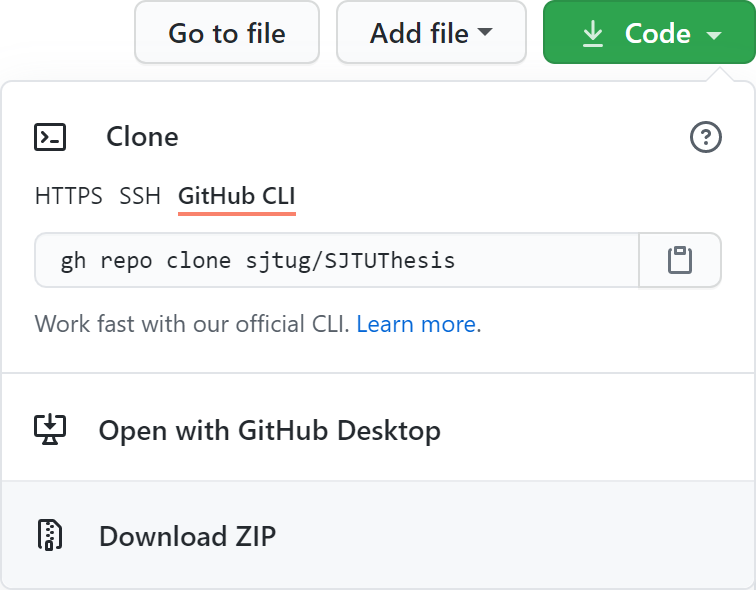
\includegraphics[width=\textwidth]{sjtuthesis-download.png}
      \end{figure}
      \vfill
    \end{column}
  \end{columns}
\end{frame}

\begin{frame}[fragile]{模板选项}
  \begin{description}
    \item[type] 指定论文类型(本科/硕士/博士)
          \begin{lstlisting}[basicstyle=\ttfamily]
\documentclass[type=bachelor]{sjtuthesis}
  \end{lstlisting}
    \item[review] 开启盲审模式
          \begin{lstlisting}[basicstyle=\ttfamily]
\documentclass[type=master,review]{sjtuthesis}
  \end{lstlisting}
    \item[fontset] 指定字体(推荐使用 \verb|windows|)
          \begin{lstlisting}[basicstyle=\ttfamily]
\documentclass[type=doctor,fontset=windows]{sjtuthesis}
  \end{lstlisting}
  \end{description}
\end{frame}

\begin{frame}[fragile]{模板设置}
  使用 \verb|\sjtusetup| 命令指定论文各类设置:
  \begin{lstlisting}
\sjtusetup{
  info = {
    zh/title  = {上海交通大学学位论文 \LaTeX{} 模板示例文档},
    en/title  = {A Sample for \LaTeX-based SJTU Thesis Template},
    zh/author = {某\quad{}某},
    en/author = {Mo Mo},
  },
  style = {
    title-logo-color = red,
  },
  name = {
    achv = {攻读学位期间完成的论文},
  },
}
  \end{lstlisting}
\end{frame}

\begin{frame}[fragile]{信息录入}
  \verb|info| 域完成论文基本信息录入
  \begin{table}[h]
    \centering
    \footnotesize
    \begin{tabular}{lll} \toprule
      命令作用   & 中文对应选项                            & 英文对应选项                       \\ \midrule
      论文标题   & \texttt{zh/title}                 & \texttt{en/title}            \\
      关键字列表  & \texttt{zh/keywords}              & \texttt{en/keywords}         \\
      作者姓名   & \texttt{zh/author}                & \texttt{en/author}           \\
      申请学位名称 & \texttt{zh/degree}                & \texttt{en/degree}           \\
      院系名称   & \texttt{zh/department}            & \texttt{en/department}       \\
      专业名称   & \texttt{zh/major}                 & \texttt{en/major}            \\
      导师     & \texttt{zh/supervisor}            & \texttt{en/supervisor}       \\
      副导师    & \texttt{zh/assoc-supervisor}      & \texttt{en/assoc-supervisor} \\
      联培导师   & \texttt{zh/co-supervisor}         & \texttt{en/co-supervisor}    \\
      日期     & \multicolumn{2}{c}{\texttt{date}}                                \\
      学号     & \multicolumn{2}{c}{\texttt{id}}                                  \\ \bottomrule
    \end{tabular}
  \end{table}
\end{frame}

\begin{frame}[fragile]{数学}
  \begin{itemize}
    \item 公式示例:\verb|contents/math_and_citations.tex|
          \link{https://github.com/sjtug/SJTUThesis/blob/master/contents/math_and_citations.tex}
    \item \SJTUThesis{} 定义了常用的数学环境(需要手工引入 \verb|amsthm| 宏包):
          \begin{table}[h]
            \centering
            \footnotesize
            \begin{tabular}{*{7}{l}}\toprule
              assumption & axiom    & conjecture & corollary   & definition &
              example    & exercise
              \\
              假设         & 公理       & 猜想         & 推论          & 定义         & 例 & 练习
              \\\midrule
              lemma      & problem  & proof      & proposition & remark     &
              solution   & theorem
              \\
              引理         & 问题       & 证明         & 命题          & 注          & 解 &
              定理
              \\\bottomrule
            \end{tabular}
          \end{table}
  \end{itemize}
\end{frame}

\begin{frame}[fragile]{参考文献}
  \begin{itemize}
    \item 建议自动生成
          \begin{itemize}
            \item \LaTeX 引擎自身不能处理参考文献,需要借助外部程序!
          \end{itemize}
    \item 传统方法:\BibTeX 后端
          \begin{itemize}
            \item 控制文献、引用样式:\pkg{natbib} 宏包
            \item 国标样式:\pkg{gbt7714} 宏包
                  \link{https://mirrors.sjtug.sjtu.edu.cn/ctan/biblio/bibtex/contrib/gbt7714/gbt7714.pdf}
          \end{itemize}
    \item 现代方法:\verb|biber| 后端 + \pkg{biblatex} 宏包
          \begin{itemize}
            \item 国标样式:\pkg{biblatex-gbt7714-2015} 宏包
                  \link{https://mirrors.sjtug.sjtu.edu.cn/ctan/macros/latex/contrib/biblatex-contrib/biblatex-gb7714-2015/biblatex-gb7714-2015.pdf}
          \end{itemize}
    \item 需要多轮编译——再次推荐 latexmk
  \end{itemize}
\end{frame}

\begin{frame}[fragile]{参考文献(续)}
  \begin{itemize}
    \item 生成 \verb|.bib| 数据库
          \begin{itemize}
            \item Google Scholar 可直接复制或者批量导出
            \item 用 Zotero、Jabref 等文献管理软件生成
          \end{itemize}
    \item 两种引用模式:
          \begin{itemize}
            \item 上标模式:如“在许多文献\textsuperscript{[12-13]}中……”
                  \begin{lstlisting}[basicstyle=\ttfamily]
    \cite{key12, key13}
          \end{lstlisting}
            \item 正文模式:如“文献~[14] 证明了……”
                  \begin{lstlisting}[basicstyle=\ttfamily,morekeywords={parencite}]
    \parencite{key14}
          \end{lstlisting}
          \end{itemize}
  \end{itemize}
\end{frame}

\begin{frame}[fragile]{\SJTUThesis 问题}
  \begin{itemize}
    \item 常见问题
          \begin{itemize}
            \item 参考文献列表出错、缺少字体、无法编译、格式不对……
            \item 阅读模板文档 \verb|sjtutex.pdf| \link{https://github.com/sjtug/SJTUTeX/releases}
                  和 SJTUThesis 示例文档代码
            \item 查看 Wiki \link{https://github.com/sjtug/SJTUThesis/wiki}
          \end{itemize}

    \item 主动提问
          \begin{itemize}
            \item GitHub Discussions 提问:\link{https://github.com/sjtug/SJTUThesis/discussions}
            \item GitHub Issues 报告 BUG:\link{https://github.com/sjtug/SJTUThesis/issues}
          \end{itemize}

  \end{itemize}
\end{frame}
